\subsection{Membres de groupe}

Nous somme trois étudiants du groupe M2:
\begin{dinglist}{111}
    \item Ying LIU
    \item Philippe NEGREL-JERZY
    \item Sébastien PONT
\end{dinglist}

\subsection{Présentation}

Nous ne représentons pas tout le sujet (que vous pouvez retrouver \href{https://spont.me/mjxoog}{ici}\footnote{\href{https://spont.me/mjxoog}{https://spont.me/mjxoog}}), mais voici un résumé.

Linda est un service permettant de partager des données sous formes de \iCode{Tuple}.
Dans ce projet nous allons implémenter deux manières de partager et gérer ces ressources à travers plusieurs clients :

\begin{itemize}
    \item une version dite "locale" à base de mémoire partagée (\iCode{shm} package Figure \ref{fig:main_class_diagram})
    \item un version dite "distante" à base de clients / mono-serveur (\iCode{server} package Figure \ref{fig:main_class_diagram})
\end{itemize}

\begin{figure}[H]
    \centering
    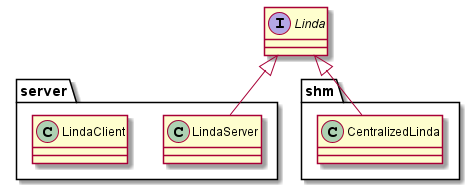
\includegraphics[scale=0.7]{src/part-01/mainCD.png}
    \caption{Diagramme de classe général du projet} \label{fig:main_class_diagram}
\end{figure}

\begin{dinglist}{111}
    \item Versio mémoire partagée (version locale) :
    \item
    \item Version client / mono-serveur (version distante)
\end{dinglist}